%!TEX root = ../thesis.tex

\section{実環境に似たシミュレータ環境による実験}
これまでの実験では, 簡易的なシミュレータ環境を用いてきた. しかし, 実験に簡易的なシミュレータ環境を用いるには問題があり, 以下の点である.

\begin{itemize}
  % \item 屋内を模している環境であるため, 影は少ないはずだが, \figref{Fig:sim_shadow}に示すように全体的に影が写り込んでしまっている

  % \begin{figure}[hbtp]
  %   \centering
  %  \includegraphics[keepaspectratio, scale=0.37]
  %       {images/sim_up.png}
  %  \caption{Ratio of data by distance from target path in test phase}
  %  \label{Fig:sim_up}
  % \end{figure} 

  % \begin{figure}[h]
  %   \centering
  %   \begin{minipage}[b]{67mm}
  %     \centering
  %     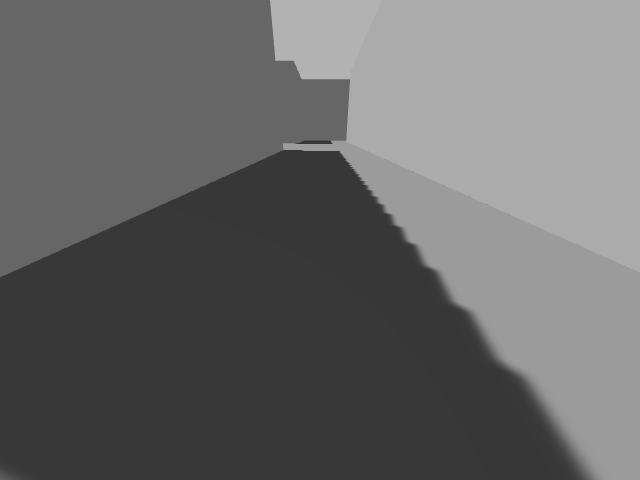
\includegraphics[width=67mm, height=50.5mm]{images/sim_robot.png}
  %     \caption*{(a)}
  %   \end{minipage} 
  %   % \newpage
  %   % \hspace{0.03\columnwidth}
  %   \begin{minipage}[b]{67mm}
  %     \centering
  %     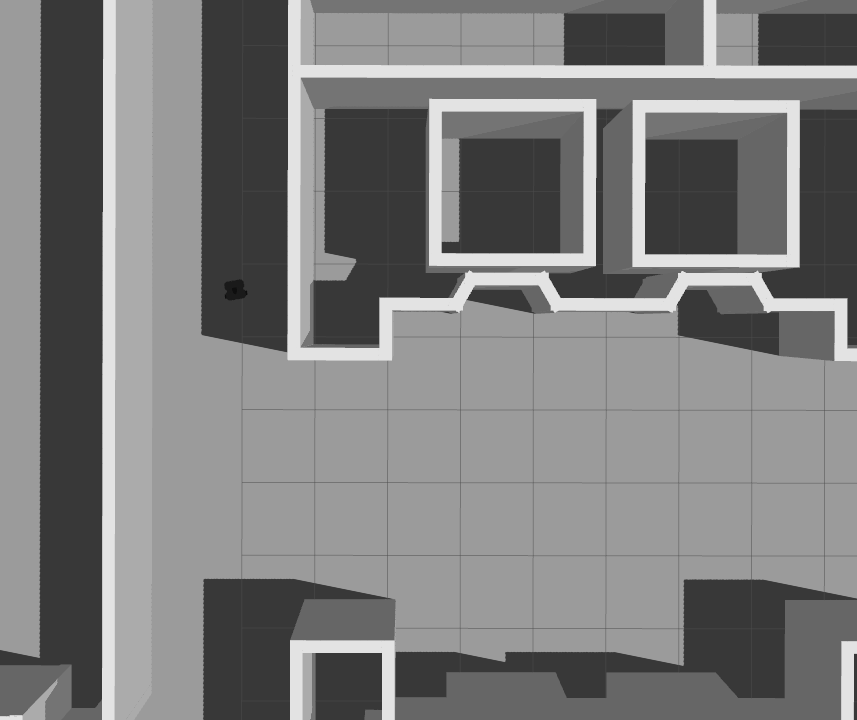
\includegraphics[width=67mm, height=50.5mm]{images/sim_up.png}
  %     \caption*{(b)}
  %   \end{minipage}
  %   \caption{Number of data per command per 10000steps in conventional experiments}
  %   \label{Fig:sim_shadow}
  % \end{figure}

  \item \figref{Fig:sim_shadow} (a)に示すように, 環境の大半が灰色や白のみで構成されているため, \figref{Fig:sim_shadow} (b)のように視覚による特徴が乏しい. 
  
   \begin{figure}[h]
    \centering
    \begin{minipage}[b]{67mm}
      \centering
      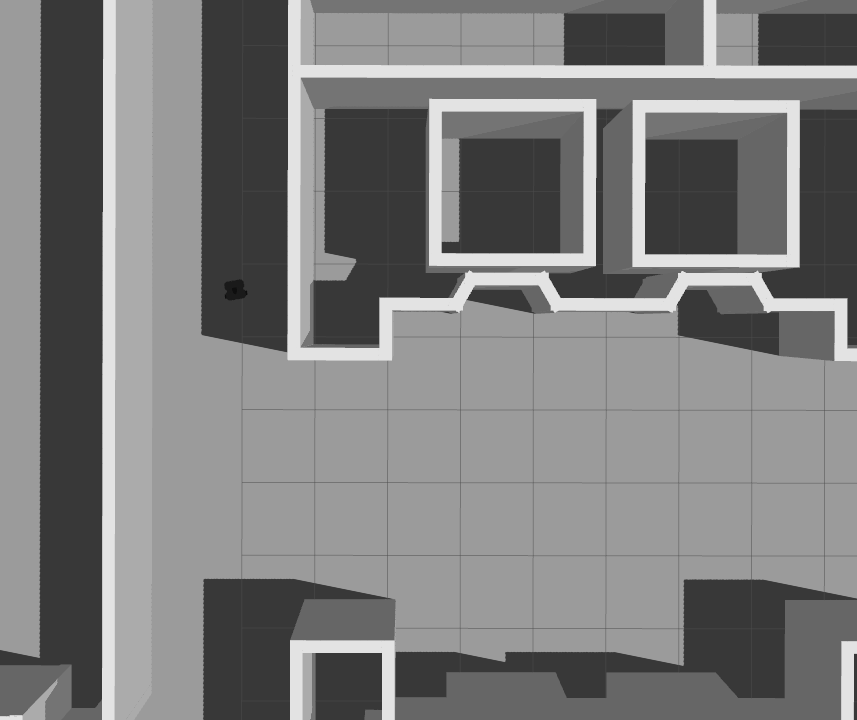
\includegraphics[width=50mm, height=36mm]{images/sim_up.png}
      \caption*{(a) A bird's eye view of the robot}
    \end{minipage} 
    % \newpage
    % \hspace{0.03\columnwidth}
    \begin{minipage}[b]{67mm}
      \centering
      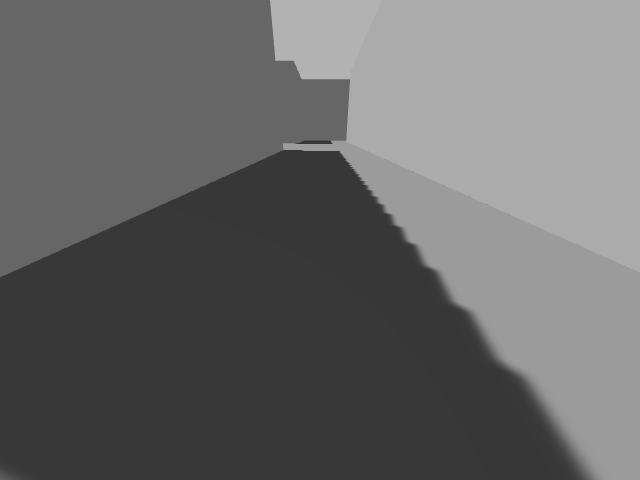
\includegraphics[width=50mm, height=36mm]{images/sim_robot.png}
      \caption*{(b) Robot Perspective}
    \end{minipage}
    \caption{Simple simulator environment}
    \label{Fig:sim_shadow}
  \end{figure}

\end{itemize}

この問題は, 学習フェーズにおいて取得するカメラ画像で学習器を訓練する際に, 大きな影響を及ぼす可能性がある. そのため, ロボットの視覚であるカメラ画像で, より多くの視覚的特徴をとらえるために, \figref{Fig:real_sim}に示すように実環境に似たシミュレータ環境を作成した. 

\begin{figure}[h]
  \centering
  \begin{minipage}[b]{67mm}
    \centering
    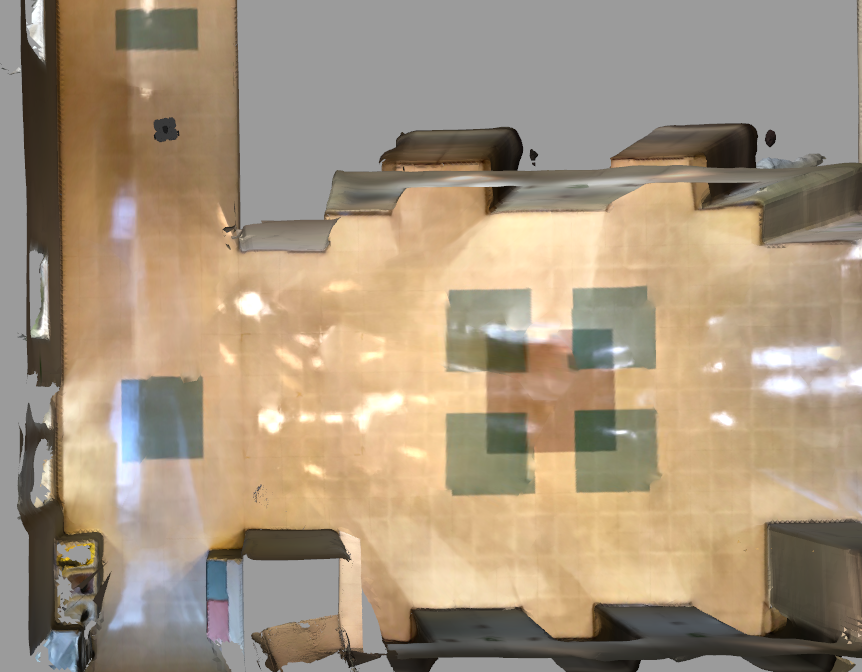
\includegraphics[width=50mm, height=36mm]{images/real_sim_up.png}
    \caption*{(a) A bird's eye view of the robot}
  \end{minipage} 
  % \newpage
  % \hspace{0.03\columnwidth}
  \begin{minipage}[b]{67mm}
    \centering
    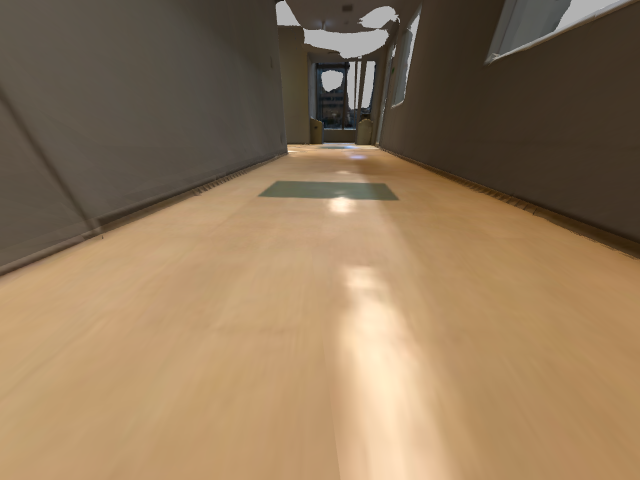
\includegraphics[width=50mm, height=36mm]{images/real_sim_robot.png}
    \caption*{(b) Robot Perspective}
  \end{minipage}
  \caption{Simulator environment similar to real environment}
  \label{Fig:real_sim}
\end{figure}

% \begin{figure}[hbtp]
%   \centering
%  \includegraphics[keepaspectratio, scale=0.8]
%       {images/RaspberryPiMouse.png}
%  \caption{Example}
%  \label{Fig:Example}
% \end{figure}

\newpage
